\documentclass[table]{beamer}

\usepackage{xcolor}
\usepackage{tikz,pgfplots,graphicx,booktabs}

\usepackage{bibentry}



\AtBeginSection[]{
    \begin{frame}
        \vfill
        \centering
        \begin{beamercolorbox}[sep=8pt,center]{title}
            \usebeamerfont{title}\insertsectionhead\par
        \end{beamercolorbox}
    \end{frame}
}

\title{Effect of Parasites on the Structure and Dynamics of Food Webs}
\author{Nicholas J. Kappler}

\date{\today}


\begin{document}
\frame{\titlepage}

\section[Outline]{}
\frame{\tableofcontents}

\section{Motivation}
%This is probably the hardest part for me. Maybe that's a bad sign.

\section{Structural Fingreprint of Parasites}

\begin{frame}
    \frametitle{Goals}
    \begin{itemize}[<+->]
        \item Look for systematic difference between parasite and free liver
            communities
        \item 
    \end{itemize}

\end{frame}

\begin{frame}
    \frametitle{6 Empirical Food Webs}
    \begin{itemize}[<+->]
        \item Intertidal ecosystems
        \item Notable for high resolution
            \begin{itemize}
                \item Between 109 and 185 trophic species 
                \item Between 840 and 2841 feeding relationships
                \item 7-9\% of possible links between species;
                    ``connectance''
                \item 17 to 68 parasite taxa, 14-46\% of species in web.
            \end{itemize}
        \item Standardized data format
    \end{itemize}
\end{frame}


\begin{frame} 
    \frametitle{Properties Considered}
    \centering
    \begin{tabular}{l r}
        \toprule
            Property&Name\\
            \midrule
            $g$&Generality\\
            $v$&Vulnerability\\
            $v_r$&Mean. Vul. Resources\\
            $g_c$&Mean. Gen. Consumers\\
            $T$&Prey-Averaged\\
            $\lambda$&Eigenvector based\\
            $C_B$,$C_{EB}$&Betweenness\\
            $\gamma^{\cdot}$&Four types of directed clustering\\
            \bottomrule
    \end{tabular}
\end{frame}

    \tikzset{littleNode/.style={circle,draw=black,inner sep =1pt,fill=white}}
    \tikzset{curvyEdge/.style={bend right = 10}}

\begin{frame}
    \frametitle{Example Food Web}
    \begin{minipage}{0.5\textwidth}
    \begin{tikzpicture}[scale=1.5]
        \draw[very thin,dashed] (0,0)--(2.75,0) node [fill=white] {$T$=1};
        \draw[very thin,dashed] (0,1)--(2.75,1) node [fill=white] {$T$=2};
        \draw[very thin,dashed] (0,2)--(2.75,2) node [fill=white] {$T$=3};
        \draw[very thin,dashed] (0,3)--(2.75,3) node [fill=white] {$T$=4};
        \draw (0.25,0) node [littleNode] (a) {1};
        \draw (1,0) node [littleNode](b) {2};
        \draw (1.75,0) node [littleNode](c) {3};
        \draw (0.25,1) node [littleNode](d) {4};
        \draw (2,1) node [littleNode](e) {5};
        \draw (1.5,1) node [littleNode](f) {6};
        \draw (1.5,2) node [littleNode](g) {7};
        \draw (2,2.5) node [littleNode](h) {8};
        \draw (1,1.75) node [littleNode](i) {9};
        \draw (0.75,2.75) node [littleNode](j) {10};
        \draw (0.75,2.75) node [littleNode](j) {10};
        \draw (0.25,2.875) node [littleNode](k) {11};
        \draw (1.5,3) node [littleNode](l) {12};
        \draw[->,>=stealth] (a) -- (d);
        \draw[->,>=stealth] (a) -- (i);
        \draw[->,>=stealth] (b) -- (i);
        \draw[->,>=stealth] (c) -- (f);
        \draw[->,>=stealth] (c) -- (e);
        \draw[->,>=stealth] (d) -- (j);
        \draw[->,>=stealth] (d) -- (k);
        \draw[->,>=stealth] (d) -- (l);
        \draw[->,>=stealth] (f) -- (i);
        \draw[->,>=stealth] (f) -- (g);
        \draw[->,>=stealth] (f) -- (h);
        \draw[->,>=stealth] (g) -- (i);
        \draw[->,>=stealth] (g) -- (h);
        \draw[->,>=stealth] (h) -- (j);
        \draw[->,>=stealth] (h) -- (l);
        \draw[->,>=stealth] (i) -- (j);
        \draw[->,>=stealth] (i) -- (l);
        \draw[->,>=stealth] (j) -- (k);
        \draw[->,>=stealth] (j) -- (l);
        \draw[->,thick,white,>=stealth,dashed] (l) to[out=140,in=60] (j);
        \only<2>{%
            \draw[->,thick,red,>=stealth] (i) -- (j);
            \draw[->,thick,red,>=stealth] (i) -- (l);
            \draw[->,thick,blue,>=stealth] (a) -- (i);
            \draw[->,thick,blue,>=stealth] (b) -- (i);
            \draw[->,thick,blue,>=stealth] (f) -- (i);
            \draw[->,thick,blue,>=stealth] (g) -- (i);
        };
    \only<3>{%
        \draw[->,red,>=stealth] (i) -- (j);
        \draw[->,red,>=stealth] (i) -- (l);
        \draw[->,thick,red,>=stealth] (j) -- (l);
        \draw[->,thick,red,>=stealth,dashed] (l) to[out=140,in=60] (j);
        \draw (0.75,2.75) node [littleNode,draw=red,thick] {\color{red}10};
        \draw (1.5,3) node [littleNode,draw = red,thick] {\color{red}12};
        \draw[->,blue,>=stealth] (a) -- (i);
        \draw[->,blue,>=stealth] (b) -- (i);
        \draw[->,blue,>=stealth] (f) -- (i);
        \draw[->,blue,>=stealth] (g) -- (i);
        \draw[->,thick,blue,>=stealth] (f) -- (g);
        \draw (0.25,0) node [littleNode,draw=blue,thick] (a) {\color{blue}1};
        \draw (1,0)    node [littleNode,draw=blue,thick] (b) {\color{blue}2};
        \draw (1.5,1)  node [littleNode,draw=blue,thick] (f) {\color{blue}6};
        \draw (1.5,2)  node [littleNode,draw=blue,thick] (g) {\color{blue}7};

    }
   \end{tikzpicture}
   \end{minipage}%
   \begin{minipage}{0.5\textwidth}
       \only<1>{\tiny
           West Coastal Tundra, Barrow, Alaska Food Web
           \begin{tabular}{r l}
               \toprule
               ID&Species Description\\
               \midrule
               1&Monocots\\
               2&Dicots\\
               3&Detritus\\
               4&Lemmings\\
               5&Microorganisms\\
               6&Saprovores\\
               7&Carnivorous Arthropods\\
               8&Shorebirds\\
               9&Longspurs\\
               10&Weasels\\
               11&Owls\\
               12&Jaegers\\
               \midrule\rowcolor{white}
               \multicolumn{2}{l}{\parbox{\linewidth}{Source: 
Cohen, J. E. (compiler) 2010  Ecologists' Co-Operative Web Bank. Version 1.1.
Machine-readable data base of food webs.  New York: The Rockefeller
University.}}\\
               \bottomrule
           \end{tabular}
       }
       \only<2>{
           Longspurs:
           \color{red}{\[v_9=2\]}
           \color{blue}{\[g_9=2\]}
           \color{black}\[T_9=\frac{1+1+2+3}{4}+1 = 2.75\]
       }
       \only<3>{
           Longspurs:
           \color{red}\[\gamma_9^c=\frac{1}{2}\]
           \color{blue}\[\gamma_9^r=\frac{1}{12}\]
           \color{black}\[\gamma_9^{rc}=\gamma^{cr}=0\]
       }
   \end{minipage}
\end{frame}

\newcommand\makeTriangleNodes[3]{%
            \draw (0,0) node [littleNode,fill=gray70] (#1) {\tiny$_i$};
            \draw (1,0) node [littleNode] (#2) {\tiny$_j$};
            \draw (.5,.866) node [littleNode] (#3) {\tiny$_k$};}
\definecolor{gray70}{gray}{.7}

%\begin{frame}
%    \frametitle{Clustering Coefficients}
%     \begin{tabular}{r c r c}
%        \toprule
%        \multicolumn{2}{l}{Consumer Clustering}&
%        \multicolumn{2}{l}{Resource Clustering}\\
%        \cmidrule(r){1-1}\cmidrule(r){3-3}
%        $\gamma_i^{c} = \frac{(A^2A^\top)_{ii}}{v_i(v_i-1)}$  
%        &\begin{tikzpicture}%Cyclic Triangle
%            \makeTriangleNodes{i}{j}{k}
%            \path [->,>=stealth]
%            (i) edge  node [right] {} (j)
%            (j) edge[gray70]  node [right] {} (k)
%            (i) edge  node [right] {} (k);
%        \end{tikzpicture}&
%        $\gamma_i^{r}= \frac{(A^\top A^2)_{ii}}{g_i(g_i-1)}$
%        &\begin{tikzpicture}%Sink 1
%            \makeTriangleNodes{i}{j}{k}
%            \path [->,>=stealth]
%            (j) edge  node [right] {} (i)
%            (j) edge[gray70]  node [right] {} (k)
%            (k) edge  node [right] {} (i);
%        \end{tikzpicture}\\
%        \midrule
%        \multicolumn{2}{l}{Resource Consumer Clustering}&
%        \multicolumn{2}{l}{Consumer Resource Clustering}\\
%        \cmidrule(r){1-1}\cmidrule(r){3-3}
%        $\gamma_i^{rc}=\frac{(AA^\top A)_{ii}}{g_iv_i-(A^2)_{ii}}$            
%        &\begin{tikzpicture}%Cyclic Triangle
%            \makeTriangleNodes{i}{j}{k}
%            \path [->,>=stealth]
%            (i) edge  node [right] {} (j)
%            (k) edge[gray70]  node [left] {} (j)
%            (k) edge   node [right] {} (i);
%        \end{tikzpicture}&
%        $\gamma_i^{cr}= \frac{(A^3)_{ii}}{g_iv_i-(A^2)_{ii}}$
%        &\begin{tikzpicture}%Cyclic Triangle
%            \makeTriangleNodes{i}{j}{k}
%            \path [->,>=stealth]
%            (i) edge node [right] {} (j)
%            (j) edge [gray70]  node [right] {} (k)
%            (k) edge  node [right] {} (i);
%        \end{tikzpicture}\\
%         \bottomrule
%    \end{tabular}
%\end{frame}

\begin{frame}
    \frametitle{Observed Patterns}
    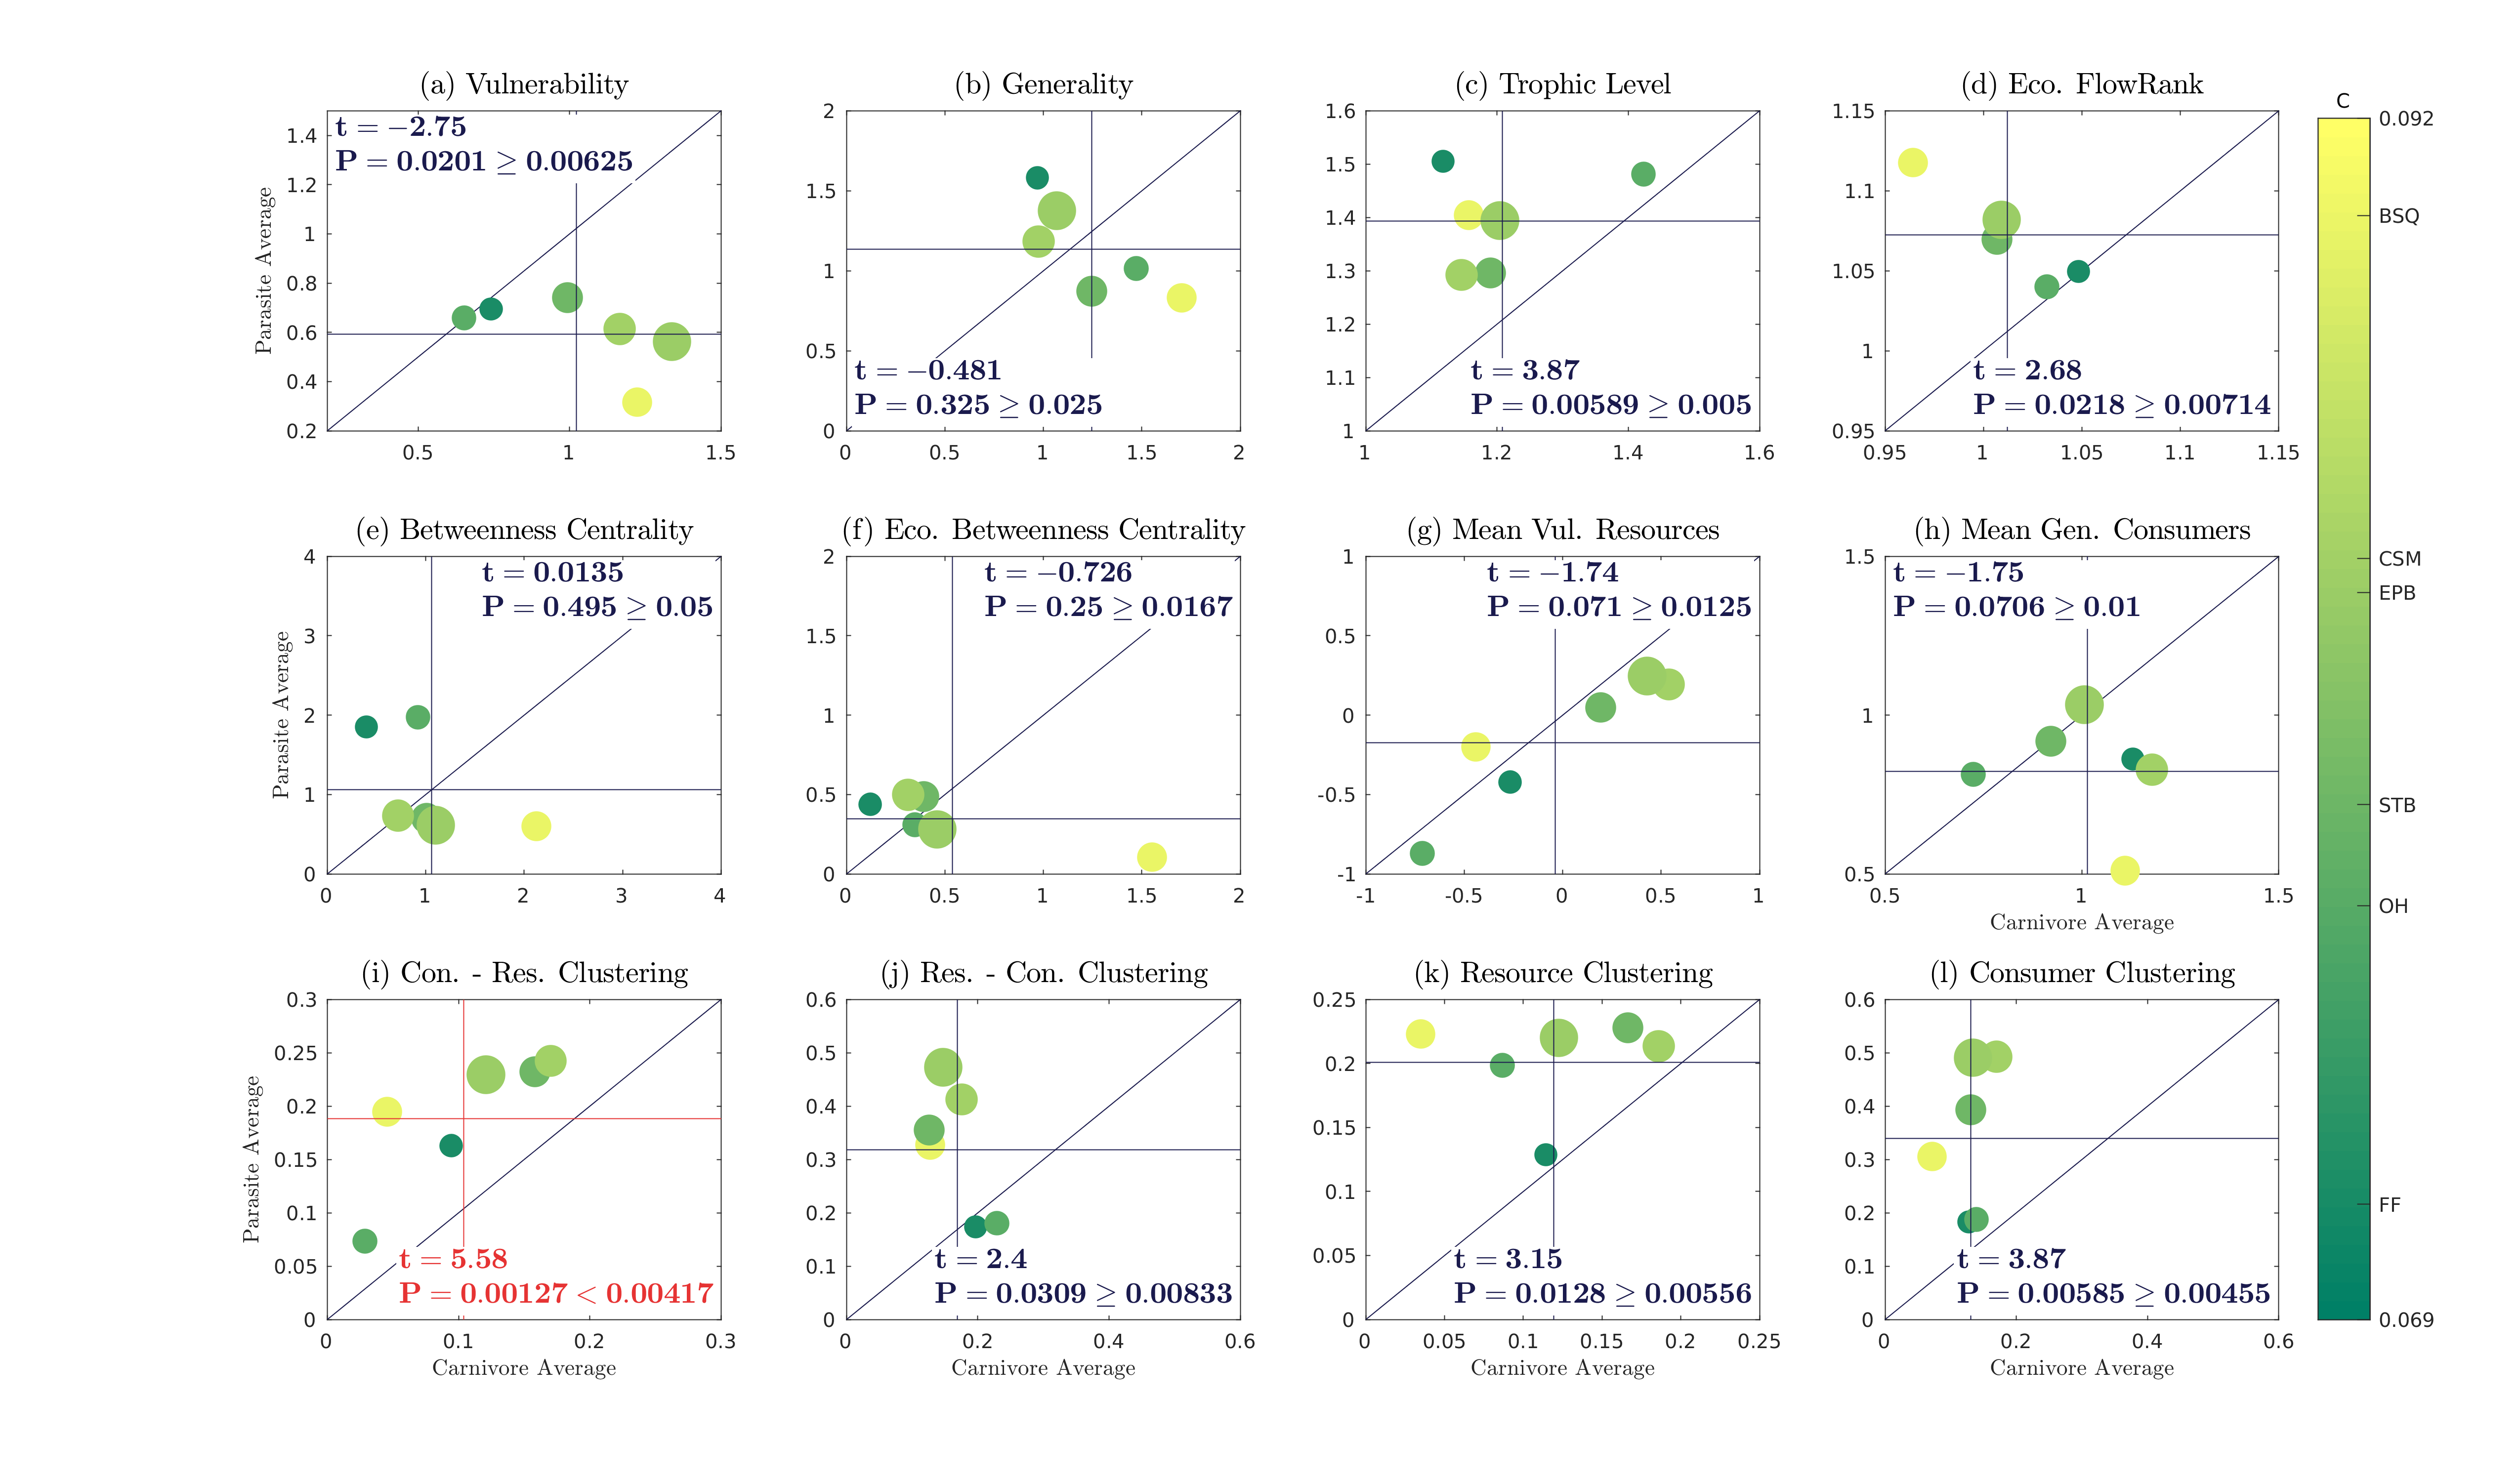
\includegraphics[width=\textwidth]{../Chapter2/figures/initialPropsMaxLinkage.png}
\end{frame}

\begin{frame}
    \frametitle{Patterns are there}
    \begin{itemize}[<+->]
        \item Network properties of individual nodes could differentiate
            parasite from free liver on about 85\% of nodes
        \item Observed patterns were robust to decreases in trophic resolution
    \end{itemize}
\end{frame}

\begin{frame}
    \frametitle{Add salt}
    \begin{itemize}[<+->]
        \item We are observing patterns in \textit{data} 
        \item Life stages were aggregated first
        \item Sampling Biases
            \begin{itemize}
                \item No parasites of plants
                \item No ectoparasites of birds, fish
                \item Poor resolution of microbes and viruses
                \item Poor resolution of Fungi
                \item Detritus as basal node
            \end{itemize}
    \end{itemize}
\end{frame}


\section{Food Web Models}

\begin{frame}
    \frametitle{Background}
    \begin{itemize}[<+->]
        \item Robert May (1972)
        \item Cohen's Cascades (1990)
        \item Niche Model (2000)
        \item Variants 
    \end{itemize}
\end{frame}

\begin{frame}
\frametitle{The Niche and Inverse Niche Models}
  \centering
    \begin{tikzpicture}
        \draw (0,0)--(10,0)
        node[anchor = west] {$n$};
        \draw (0,.2)--(0,-.2)
        node[anchor = north] {$0$};
        \draw (10,.2)--(10,-.2)
        node[anchor = north] {$1$};
        %Predator
        \fill (7,0) circle (.07) 
        node[anchor = south west]  {$n_j$};
        %Predator Diet
        \draw (7,0)--(7,.75)--(2.8,.75)--(2.8,.5);
        \draw (1.3,0) -- (1.3,.5) -- (4.3,.5) -- (4.3,0);
        \draw[dashed] (2.8,.5) -- (2.8,0) 
        node[anchor = north] {$c_j$};
        \draw[<->,>=stealth] (1.3,1.2) -- (4.3,1.2)
        node[fill=white,pos = 0.5] {$r_j$}; 
        \draw[dashed] (1.3,0.5)--(1.3,1.25);
        \draw[dashed] (4.3,0.5)--(4.3,1.25);
        %Prey
        \fill (3,0) circle (.07) 
        node[anchor = south west]  {$n_i$};
        \draw(3.4,-2) circle (.3)
        node {$i$};
        \draw[->,>=stealth] (3.7,-2) -- (4.7,-2);
        \draw(5,-2) circle (.3)
        node {$j$};
    \only<2>{ 
        %Parasite 
        \fill (1,0) circle (.07) 
        node[anchor = south]  {$n_p$};
        \draw[->,>=stealth] (5.3,-2) -- (6.3,-2);
        \draw (6.6,-2) circle (.3) node {$p$};
        \draw (1,0) -- (1,-0.75) -- (7,-0.75) -- (7,-0.5);
        \draw (5.5,0) -- (5.5,-0.5) -- (8.5,-0.5) -- (8.5,0);
        \draw[<->,>=stealth] (5.5,-1.2) -- (8.5,-1.2)
        node[fill=white,pos = 0.5] {$r_p$}; 
        \draw[dashed] (5.5,-0.5)--(5.5,-1.25);
    \draw[dashed] (8.5,-0.5)--(8.5,-1.25);}
    \end{tikzpicture}
\only<1>{
    \begin{itemize}
        \item $n_i \sim U(0,1)$
        \item $y_i \sim \text{Beta}(1,\beta)$
        \item $r_i \sim n_i \cdot y_i$
        \item $c_{i}\sim U(\max{(0,r_i/2)},\min{1-r_i/2,n_i})$
    \end{itemize}
}
\only<2>{
    \begin{itemize}
        \item $n_p \sim U(0,1)$
        \item $y_p \sim \text{Beta}(1,\beta_p)$
        \item $r_p \sim (1-n_p) \cdot y_p$
        \item $c_{p}\sim U(\{n_j|j\in\text{free livers},n_j>n_p\})$
    \end{itemize}
}
\end{frame}

\begin{frame}
    \frametitle{Models Tested}
    \begin{itemize}[<+->]
        \item Niche model with randomly chosen parasites
        \item Inverse Niche Model, matching number of links within and between
            free liver and parasite communities
            \begin{itemize}
                \item e.g. free liver - parasite more common than parasite -
                    parasite
            \end{itemize}
    \end{itemize}
\end{frame}

\begin{frame}
    \frametitle{How to Assess Fit}
    \begin{itemize}[<+->]
        \item Ensemble of food webs from each model
        \item Calculate properties
        \item Distribution of ensemble properties
        \item How many of the empirical properties are reasonable viz. ensemble
            properties?
    \end{itemize}
\end{frame}

\rowcolors{2}{white}{gray!25}
\begin{frame}
    \frametitle{Laundry List of Properties}
    \tiny
    \centering
    \begin{tabular}{l p{3in}}
        \toprule
        \rowcolor{white}Property & Definition and Comments\\
        \midrule
        \rowcolor{white}\multicolumn{2}{l}{Global and Comm. Props.}\\\cmidrule{1-1}
        Top,Int,Bas&The fraction of top, intermediate, and basal species in the
        web, respectively.\\
        Herb,Carn&The fractions of herbivores and carnivores,respectively.\\
        Omn&The fraction of species that consume both a basal and a non-basal
        species. The set $\{$Top,Int,Bas,Herb,Carn,Omn$\}$ has only
        four degrees of freedom.\\
        Cann&The fraction of cannibals in the food web.\\
        $\rho_{gv}$&The correlation between generality and vulnerability.\\
        $\sigma_{g}$&The standard deviation of generality.\\
        $\sigma_{v}$&The standard deviation of vulnerability.\\
        $T$&The mean prey-averaged trophic level.\\
        FlowRankSD&The standard deviation of the FlowRank metric.\\
        PATH&The average link distance of every species to every other.\\
        Loop&The fraction of species involved in a loop.\\
        EcoBtwn&The mean Ecological Betweenness over all species.\\
        $\gamma^{c}$, $\gamma^{r}$, $\gamma^{rc}$, and $\gamma^{cr}$.& The
        clustering coefficients \\
        MaxSim&The average of the maximum similarity of each species to all
        other species.\\
        \midrule
        \rowcolor{white}Community Properties\\\cmidrule{1-1}
        $\overline{v}$,$\overline{g}$&Mean vulnerability and mean generality.\\
        FlowRank&Based on eigenvalue of the augmented food web\\
        $C_{EB}$&Ecological Betweenness \\
        $v_r$ and $g_c$&Mean vulnerability of resources and mean generality of
        consumers.\\\bottomrule  
    \end{tabular}
\end{frame}

\begin{frame}
    \frametitle{Entire Web Results}
    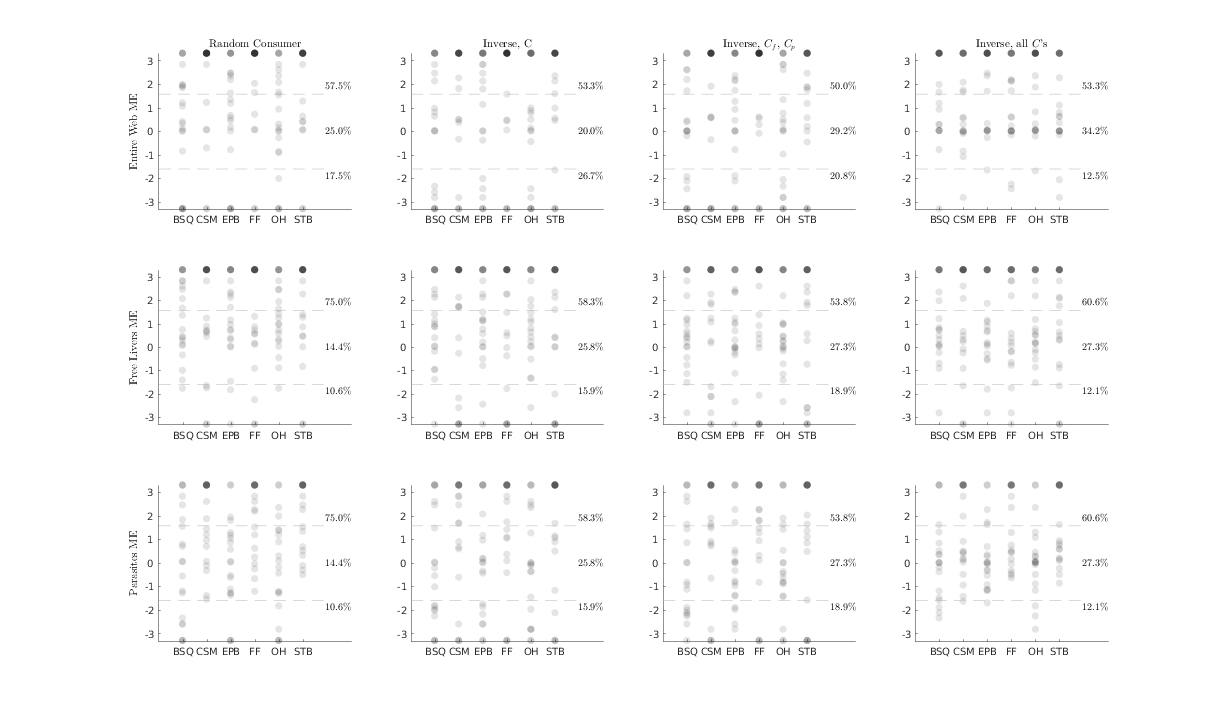
\includegraphics[width=\textwidth]{../Chapter3/figures/Properties-Raw.png}
\end{frame}

\begin{frame}
    \frametitle{Free Liver Community Results}
    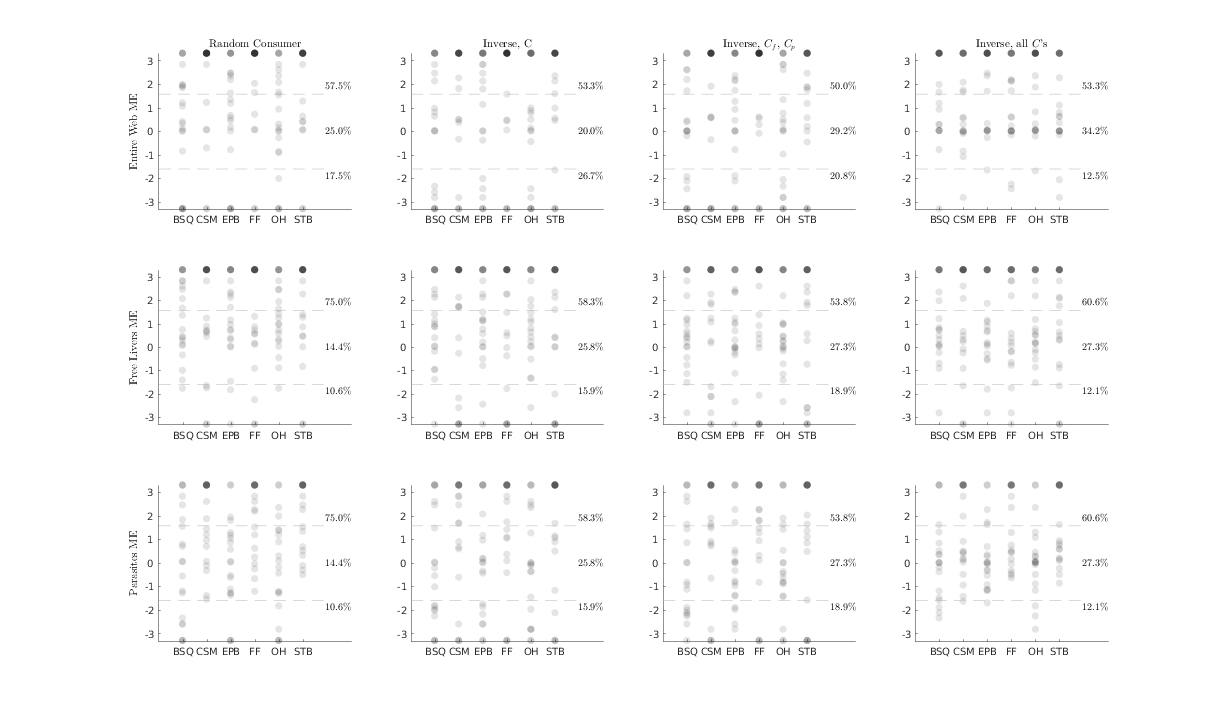
\includegraphics[width=\textwidth]{../Chapter3/figures/Properties-Raw.png}
\end{frame}

\begin{frame}
    \frametitle{Parasite Community Results}
    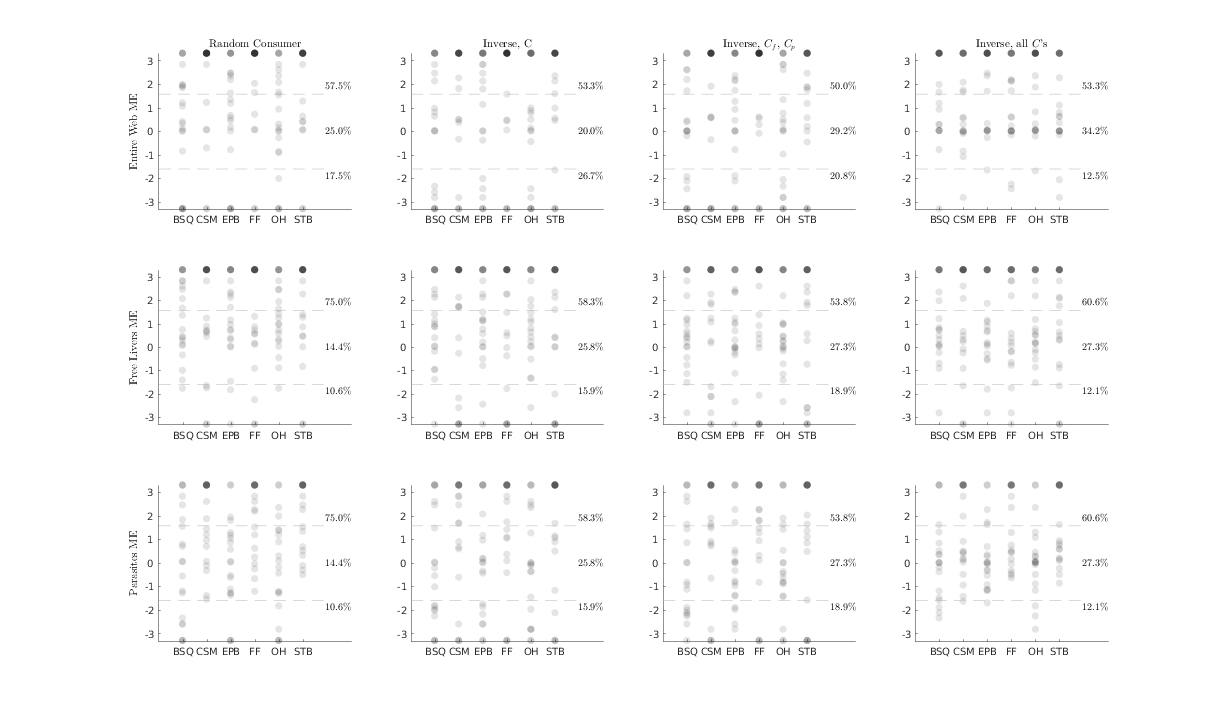
\includegraphics[width=\textwidth]{../Chapter3/figures/Properties-Raw.png}
\end{frame}

\begin{frame}
    \frametitle{Discussion}
    \begin{itemize}[<+->]
        \item Inverse niche model does better
        \item Matching subweb connectances is key
        \item Scale dependence
        \item Correlations in properties
    \end{itemize}
\end{frame}

\section{ATN Model}

\begin{frame}
    \frametitle{Allometric Trophic Network Model} 
    \begin{itemize}[<+->]
        \item All activity by a species is driven by metabolic rate
        \item Metabolic rate scales allometrically
        \item $x_i = a_{x_i}M_i^{-0.25}$
        \item Body size and body size ratios
        \item $M_i = Z^{T-1}$
    \end{itemize}
\end{frame}


\begin{frame}
    \frametitle{Equations} 
    \begin{align}
        \frac{dB_{b}}{dt} &= r_bB_b\left(1-\frac{\sum_{k\in\text{basal}}B_k}{K}\right) - \sum_kx_kB_k\frac{y_{bk}F_{bk}}{e_{bk}}\\ 
        \frac{dB_{c}}{dt} &= -x_cB_c + x_cB_c\sum_ky_{kc}F_{kc} - \sum_k x_kB_k\frac{y_{ck}F_{ck}}{e_{ck}}
    \end{align}
\end{frame}

\begin{frame}
    \frametitle{Functional Response}
    ``Attack rate on population of species $i$ by a unit of species $j$''

    \[
        F_{ij} = \frac{\omega_{ij}B_i^{1+q}}{B_0^{1+q} + \sum_k\omega_{kj}B_k^{1+q}}
    \]
\end{frame}

\begin{frame}
\frametitle{Consumer - Resource Body Size Ratio}
\begin{itemize}
\item<1-> Want parasites $Z_p$ times host and free livers $Z_f$ times resource.
\item<2-> Free liver $i$:
\[
M_i=Z_f^{T_i-1}
\]
\item<3-> $p$ parasite:
\only<3>{
Maybe...?

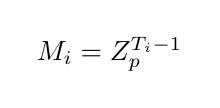
\begin{tikzpicture}
\node at (0,0) {$M_i = Z_p^{T_i-1}$};
\end{tikzpicture}
}

\only<4>{
Wrong!

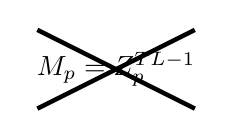
\begin{tikzpicture}
\node at (0,0) {$M_p = Z_p^{TL-1}$};
\draw [ultra thick] (-1,.5) -- (1,-.5);
\draw [ultra thick] (-1,-.5) -- (1,.5);
\end{tikzpicture}}
\end{itemize}
\end{frame}

\begin{frame}
\frametitle{Body Size Hierarchy}
\only<1>{
$Z = 10$ (no parasites):
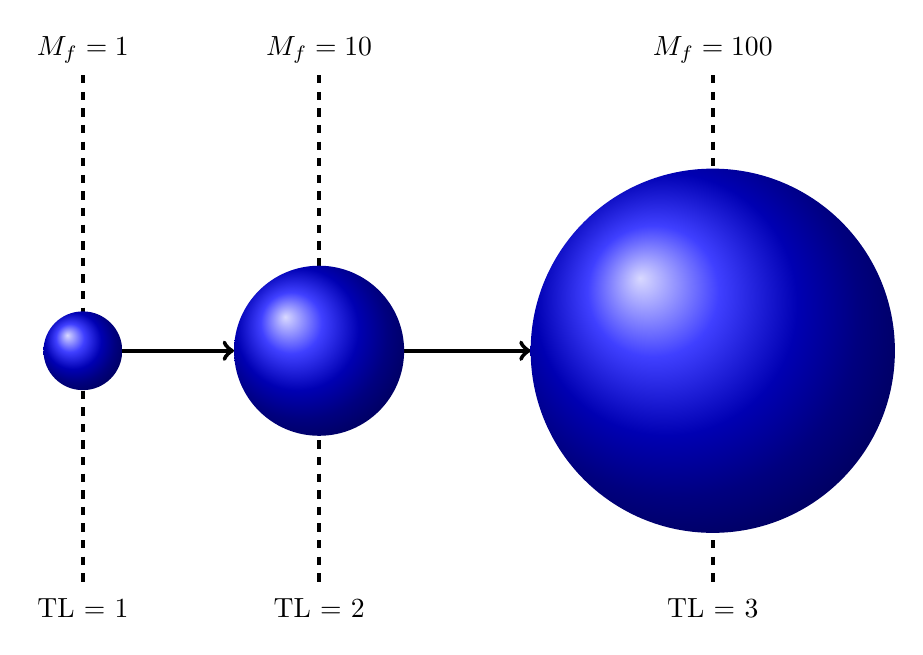
\begin{tikzpicture}
\draw[->,ultra thick] (.5,-1) -> (1.92,-1);
\draw[->,ultra thick] (4.08,-1) -> (5.687,-1);
\draw [ultra thick, dashed] (8,2.5) node [anchor = south]  {$M_f = 100$}--(8,-4) node [anchor = north] {TL = 3};
\draw [ultra thick, dashed] (3,2.5) node [anchor = south]  {$M_f = 10$}--(3,-4) node [anchor = north] {TL = 2};
\draw [ultra thick, dashed] (0,2.5) node [anchor = south]  {$M_f = 1$}--(0,-4) node [anchor = north] {TL = 1};
\shade [ball color=blue] (0,-1) circle (.5cm);
\shade [ball color=blue] (3,-1) circle (1.08cm);
\shade [ball color=blue] (8,-1) circle (2.313cm);
\end{tikzpicture}
}
\only<2>{
$Z = 10$ (no parasites):
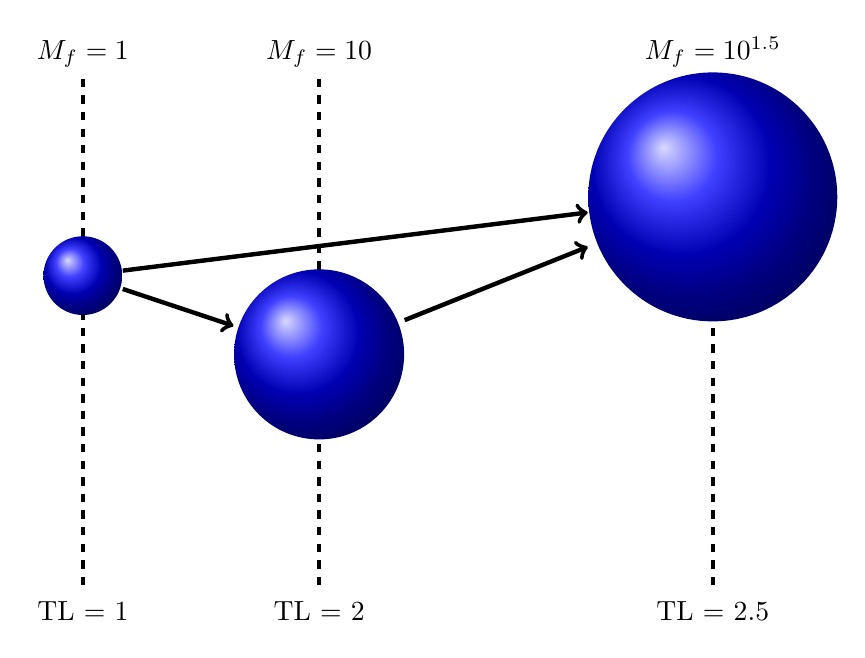
\begin{tikzpicture}
\node [inner sep = .5cm] (s1) at (0,0) {};
\node [inner sep = 1.08cm] (s2) at (3,-1) {};
%\node [inner sep = 2.313cm] (s3) at (8,1) {};
\node [inner sep = 1.581cm] (s4) at (8,1) {};
\draw[->,ultra thick] (s1) -> (s2);
%\draw[->,ultra thick] (s2) -> (s3);
\draw[->,ultra thick](s1) -> (s4);
\draw[->,ultra thick](s2) -> (s4);
\draw [ultra thick, dashed] (8,2.5) node [anchor = south]  {$M_f = 10^{1.5}$}--(8,-4) node [anchor = north] {TL = 2.5};
%\draw [ultra thick, dashed] (8,2.5) node [anchor = south]  {$M_f = 100$}--(8,-4) node [anchor = north] {TL = 3};
\draw [ultra thick, dashed] (3,2.5) node [anchor = south]  {$M_f = 10$}--(3,-4) node [anchor = north] {TL = 2};
\draw [ultra thick, dashed] (0,2.5) node [anchor = south]  {$M_f = 1$}--(0,-4) node [anchor = north] {TL = 1};
\shade [ball color=blue] (s1) circle (.5cm);
\shade [ball color=blue] (s2) circle (1.08cm);
%\shade [ball color=blue] (s3) circle (2.313cm);
\shade [ball color=blue] (s4) circle (1.581cm);
\end{tikzpicture}
}
\only<3>{
    $Z_f=10$, $Z_p = 10^{-3}$
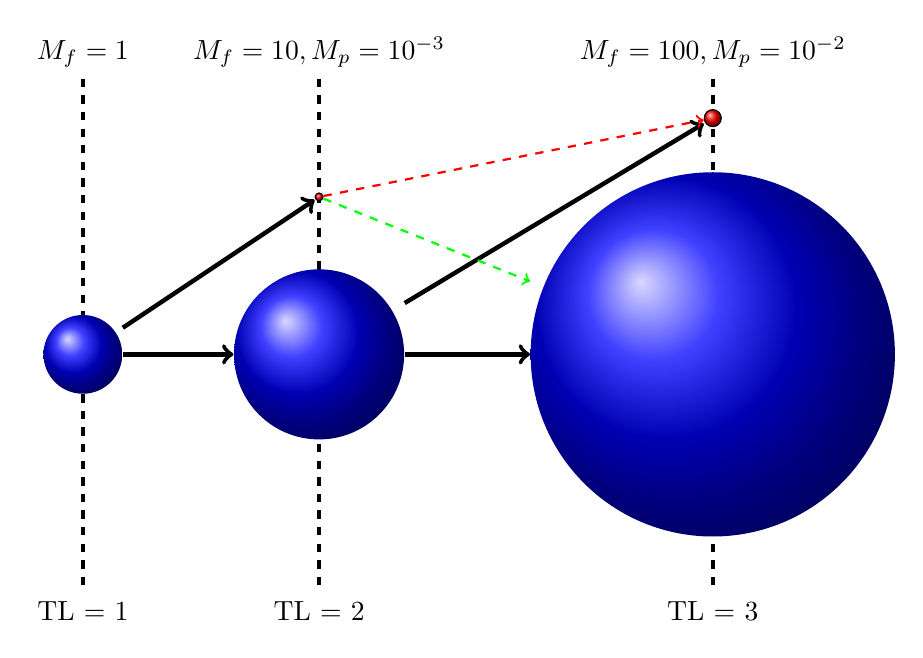
\begin{tikzpicture}
\node [inner sep = .05cm] (p1) at (3,1) {};
\node [inner sep = .108cm] (p2) at (8,2) {};
\node [inner sep = .5cm] (s1) at (0,-1) {};
\node [inner sep = 1.08cm] (s2) at (3,-1) {};
\node [inner sep = 2.313cm] (s3) at (8,-1) {};
\draw[->,ultra thick] (s1) -> (s2);
\draw[->,ultra thick] (s2) -> (s3);
\draw [ultra thick, dashed] (8,2.5) node [anchor = south]  {$M_f = 100,M_p=10^{-2}$}--(8,-4) node [anchor = north] {TL = 3};
\draw [ultra thick, dashed] (3,2.5) node [anchor = south]  {$M_f = 10,M_p=10^{-3}$}--(3,-4) node [anchor = north] {TL = 2};
\draw [ultra thick, dashed] (0,2.5) node [anchor = south]  {$M_f = 1$}--(0,-4) node [anchor = north] {TL = 1};
\draw[->,ultra thick] (s1) -> (p1);
\draw[->,ultra thick] (s2) -> (p2);
\draw[->,dashed,thick,red] (p1) -> (p2);
\draw[->,dashed,thick,green] (p1) -> (s3);
\shade [ball color=blue] (s1) circle (.5cm);
\shade [ball color=blue] (s2) circle (1.08cm);
\shade [ball color=blue] (s3) circle (2.313cm);
\draw [ball color=red] (p1) circle (.05cm);
\draw [ball color = red] (p2) circle (.108cm);
\end{tikzpicture}
}
\end{frame}

\begin{frame}
\frametitle{Consumer - Resource Body Size Ratio}
\begin{itemize}[<+->]
\item If $p$ and $k$: exponents of body size ratios of parasite-host and
    consumer-resource relationships,
\item $i$ free liver:
\[
M_i = 10^{k(T_i-1)}
\]
\item $i$ parasite:
\[
M_i = 10^{p + k(T_i-2)}
\]
\end{itemize}
\end{frame}

\begin{frame}
    \frametitle{Modifications to ATN}
    \begin{itemize}[<+->]
        \item Concomittant predation
        \item Fraction of biomass outside host, $\phi_i$
        \item \color{red} Concomittant Diagram
        \item \color{red}Cartoon of models
    \end{itemize}
\end{frame}

\begin{frame}
    \frametitle{Parasite Model}
    \begin{align*}
        \frac{dB_{b}}{dt} =
        r_bB_b\left(1-\frac{\sum_{k\in\text{basal}}B_k}{K}\right) &-
        \sum_k\phi_kB_kx_k\frac{y_{bk}^{}F_{bk}^{(troph)}}{e_{bk}}\\ & - \sum_k(1-\phi_k)B_kx_k\frac{y_{bk}^{}F^{(para)}_{bk}}{e_{bk}}
    \end{align*}
    \begin{align*}
        \frac{dB_{c}}{dt} &= -x_cB_c + \phi_cx_cB_c\sum_ky_{kc}^{ }F^{(troph)}_{kc} + (1-\phi_c)x_cB_c\sum_ky_{kc}^{ }F^{(para)}_{kc}\\ 
        & - \sum_k \phi_kx_kB_k\frac{y_{ck}^{}F^{(troph)}_{ck}}{e_{ck}} -
        \sum_k (1-\phi_k)x_kB_k\frac{y_{ck}^{}F^{(para)}_{ck}}{e_{ck}} - C_p
    \end{align*}
\end{frame}

\begin{frame}
    \frametitle{New Functional Response}
    \[
        F_{ij}^{(troph)} = \frac{\omega_{ij}^{(troph)}(\phi_iB_i)^{1+q}}{B_0^{1+h} + \sum_k\omega^{(troph)}_{kj}(\phi_kB_k)^{1+q}} \label{subeq:fr1troph}
    \]
    \[
        F_{ij}^{(para)} = \frac{\omega_{ij}^{(para)}(\phi_iB_i)^{1+h}}{B_0^{1+q} + \sum_k\omega^{(para)}_{kj}(\phi_kB_k)^{1+q}} 
    \]
\end{frame}

\begin{frame}
    \frametitle{Concomittant Losses}
    \begin{itemize}[<+->]
        \item \[C_p = \sum_ha_{ph}L_h  \]
        \item 
            \[ a_{ph} =
            \frac{(1-\phi_p)B_p}{B_h}\frac{y_{hp}^{}F_{hp}^{(para)}}{\sum_{k}y_{kp}^{}F^{(para)}_{kp}}\] 
        \item \[ 
            L_h = \sum_kx_kB_k\frac{y^{}_{kh}F^{(troph)}_{kh}}{e^{}_{kh}}\] 
    \end{itemize}
\end{frame}

\begin{frame}
    \frametitle{Results of Simulations: Null Model}
    \centering
    \includegraphics[width=.7\textwidth]{../Chapter4/figures2/pdf/null-smallFree.pdf}
\end{frame}

\begin{frame}
    \frametitle{Discussion}
    \begin{itemize}[<+->]
        \item Parasites are destabilizing
        \item Parasite model doesn't help
        \item Larger free livers do worse
        \item Separation of time scales is likely key
           %Diagram of what I think might be happening?
    \end{itemize}
\end{frame}

\begin{frame}
    \frametitle{Takeaway}
    \begin{itemize}[<+->]
        \item Data say there are structural patterns of parasite community 
        \item Those patterns are better matched by inverse niche model, but not as
            well as free livers are by the niche model
        \item Simple integration of parasite metabolic rates doesn't work that
            well in the ATN
    \end{itemize}
\end{frame}

\begin{frame}
    \frametitle{Next Steps}
    \begin{itemize}[<+->]
        \item Try ATN with inverse niche models
        \item Verify proposed mechanism of extinctions in ATN
    \end{itemize}
\end{frame}

\bibliographystyle{siam}
\bibliography{../Bib_green.bib}

\end{document}
